
The openETCS system contains two APIs:
\begin{enumerate}
\item \emph{openETCS API}: the interface specification between the
EVC platform and the openETCS application;
\item \emph{Model API}: the interface between the model itself written in
SCADE and the surrounding runtime. Both the SCADE model and the
runtime are making the openETCS application.
\end{enumerate}

\begin{figure}[h]
\centering
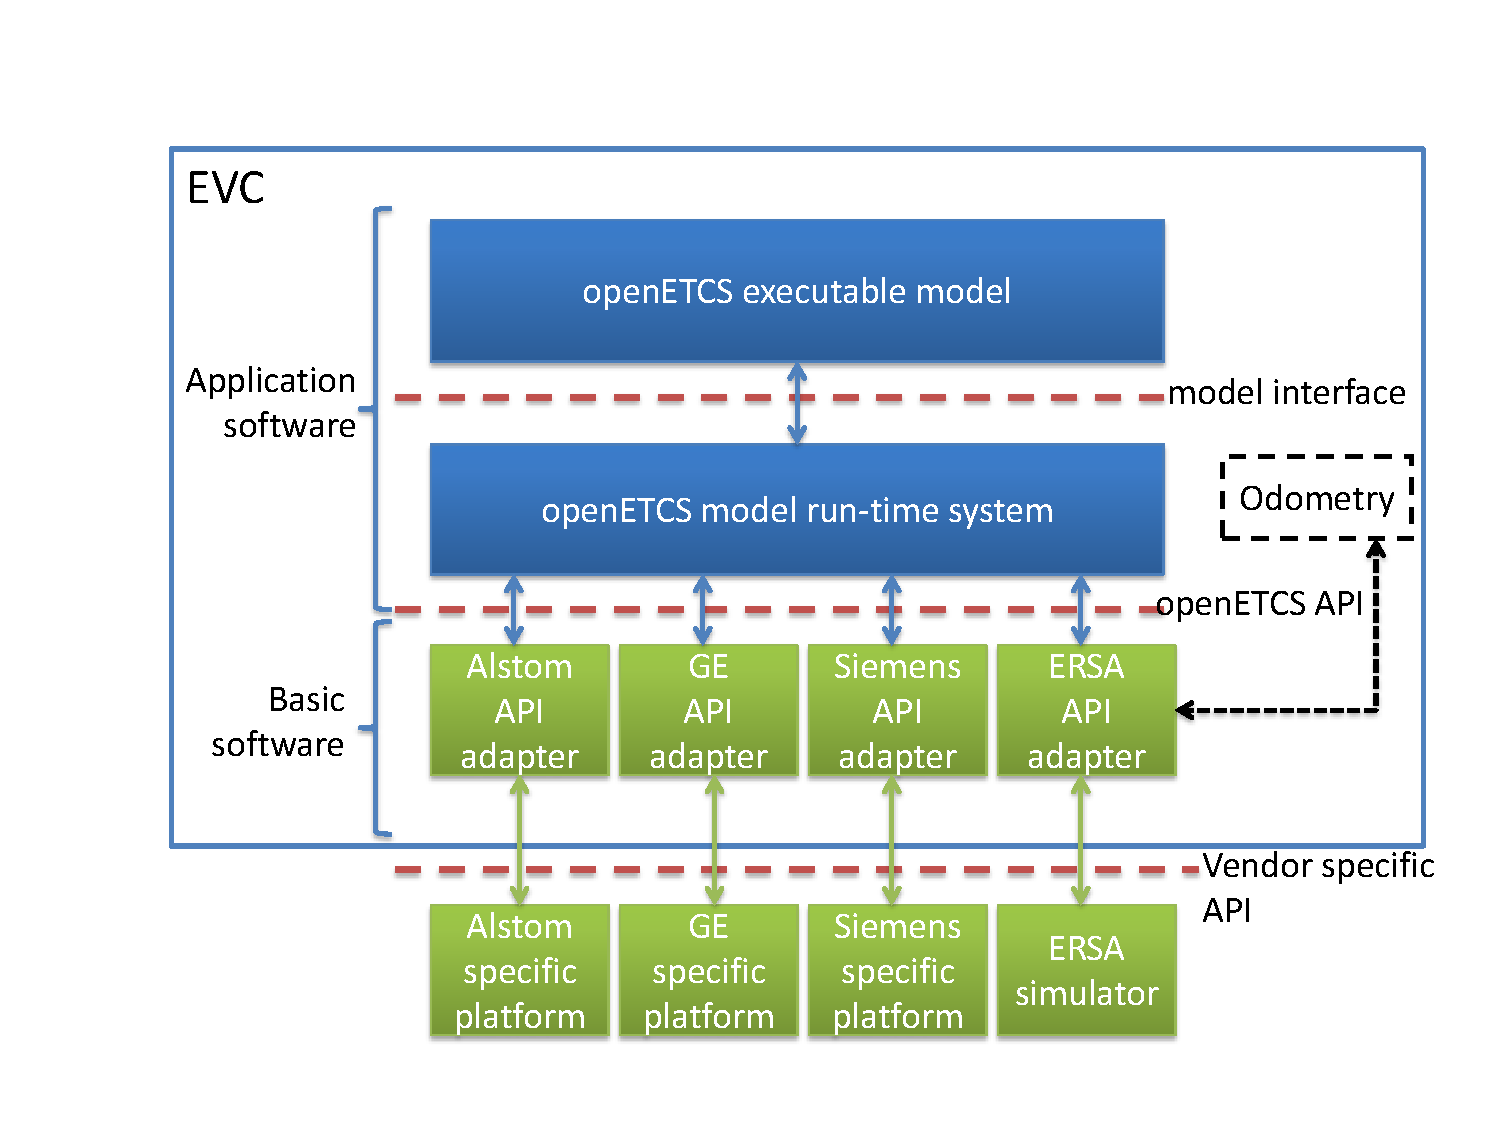
\includegraphics[width=\textwidth]{software-architecture.pdf}
\caption{openETCS software architecture}
\label{fig:software-architecture}
\end{figure}

Figure \ref{fig:software-architecture} shows both openETCS API and
model API on the software stack.

\subsection{openETCS API}

The openETCS API is currently defined by two documents, one written by
Alstom \cite{alstom-api} and a more abstract specification written by
openETCS members \cite{openetcs-api}.

The openETCS API defines the interfaces between the EVC platform and
the openETCS application for the following units surrounding the EVC:
\begin{itemize}
\item TIU (Train Interface Unit),
\item ODO (Odometry),
\item DMI (Driver Machine Interface);
\item STM (Specific Transmission Module, up to 8 units),
\item BTM (Balise Transmission Module),
\item LTM (Loop Transmission Module),
\item EURORADIO,
\item JRU (Juridical Recording Unit), and
\item zero or more vendor specific units.
\end{itemize}
Note: in the scope of the first iteration the following interfaces are used: BTM, ODO, 

The presence of intefaces to TIU, DMI and EURORADIO is visible in the interfaces, but not coded.


\subsection{Model API}

The model API is currently defined by the inputs and outputs of the SCADE model (ReceiveBaliseFromAPI).

For the proper working of the SCADE model, a set of assumptions are assumed:
\begin{itemize}
\item \textbf{Eurobalise (BTM)}: It is assumed that at most one
``telegram'' is provided per call of the SCADE model. This
``telegram'' is the merge of the telegrams of the balises making a
balise group.
\end{itemize}

% LocalWords:  SCADE API openETCS Alstom EVC EURORADIO Odometry balises balise
